\documentclass{article}

\usepackage{graphicx}
\usepackage{tikz}
\usepackage{tikzsymbols}
\usetikzlibrary{calc,patterns,shapes.geometric}
\pagestyle{empty}
\usepackage[margin=0pt]{geometry}
\geometry{papersize={14in,12in}}

\def\centerarc[#1](#2)(#3:#4:#5){\draw[#1] ($(#2)+({#5*cos(#3)},{#5*sin(#3)})$) arc (#3:#4:#5);}

\begin{document}
	\begin{figure}
		\centering
		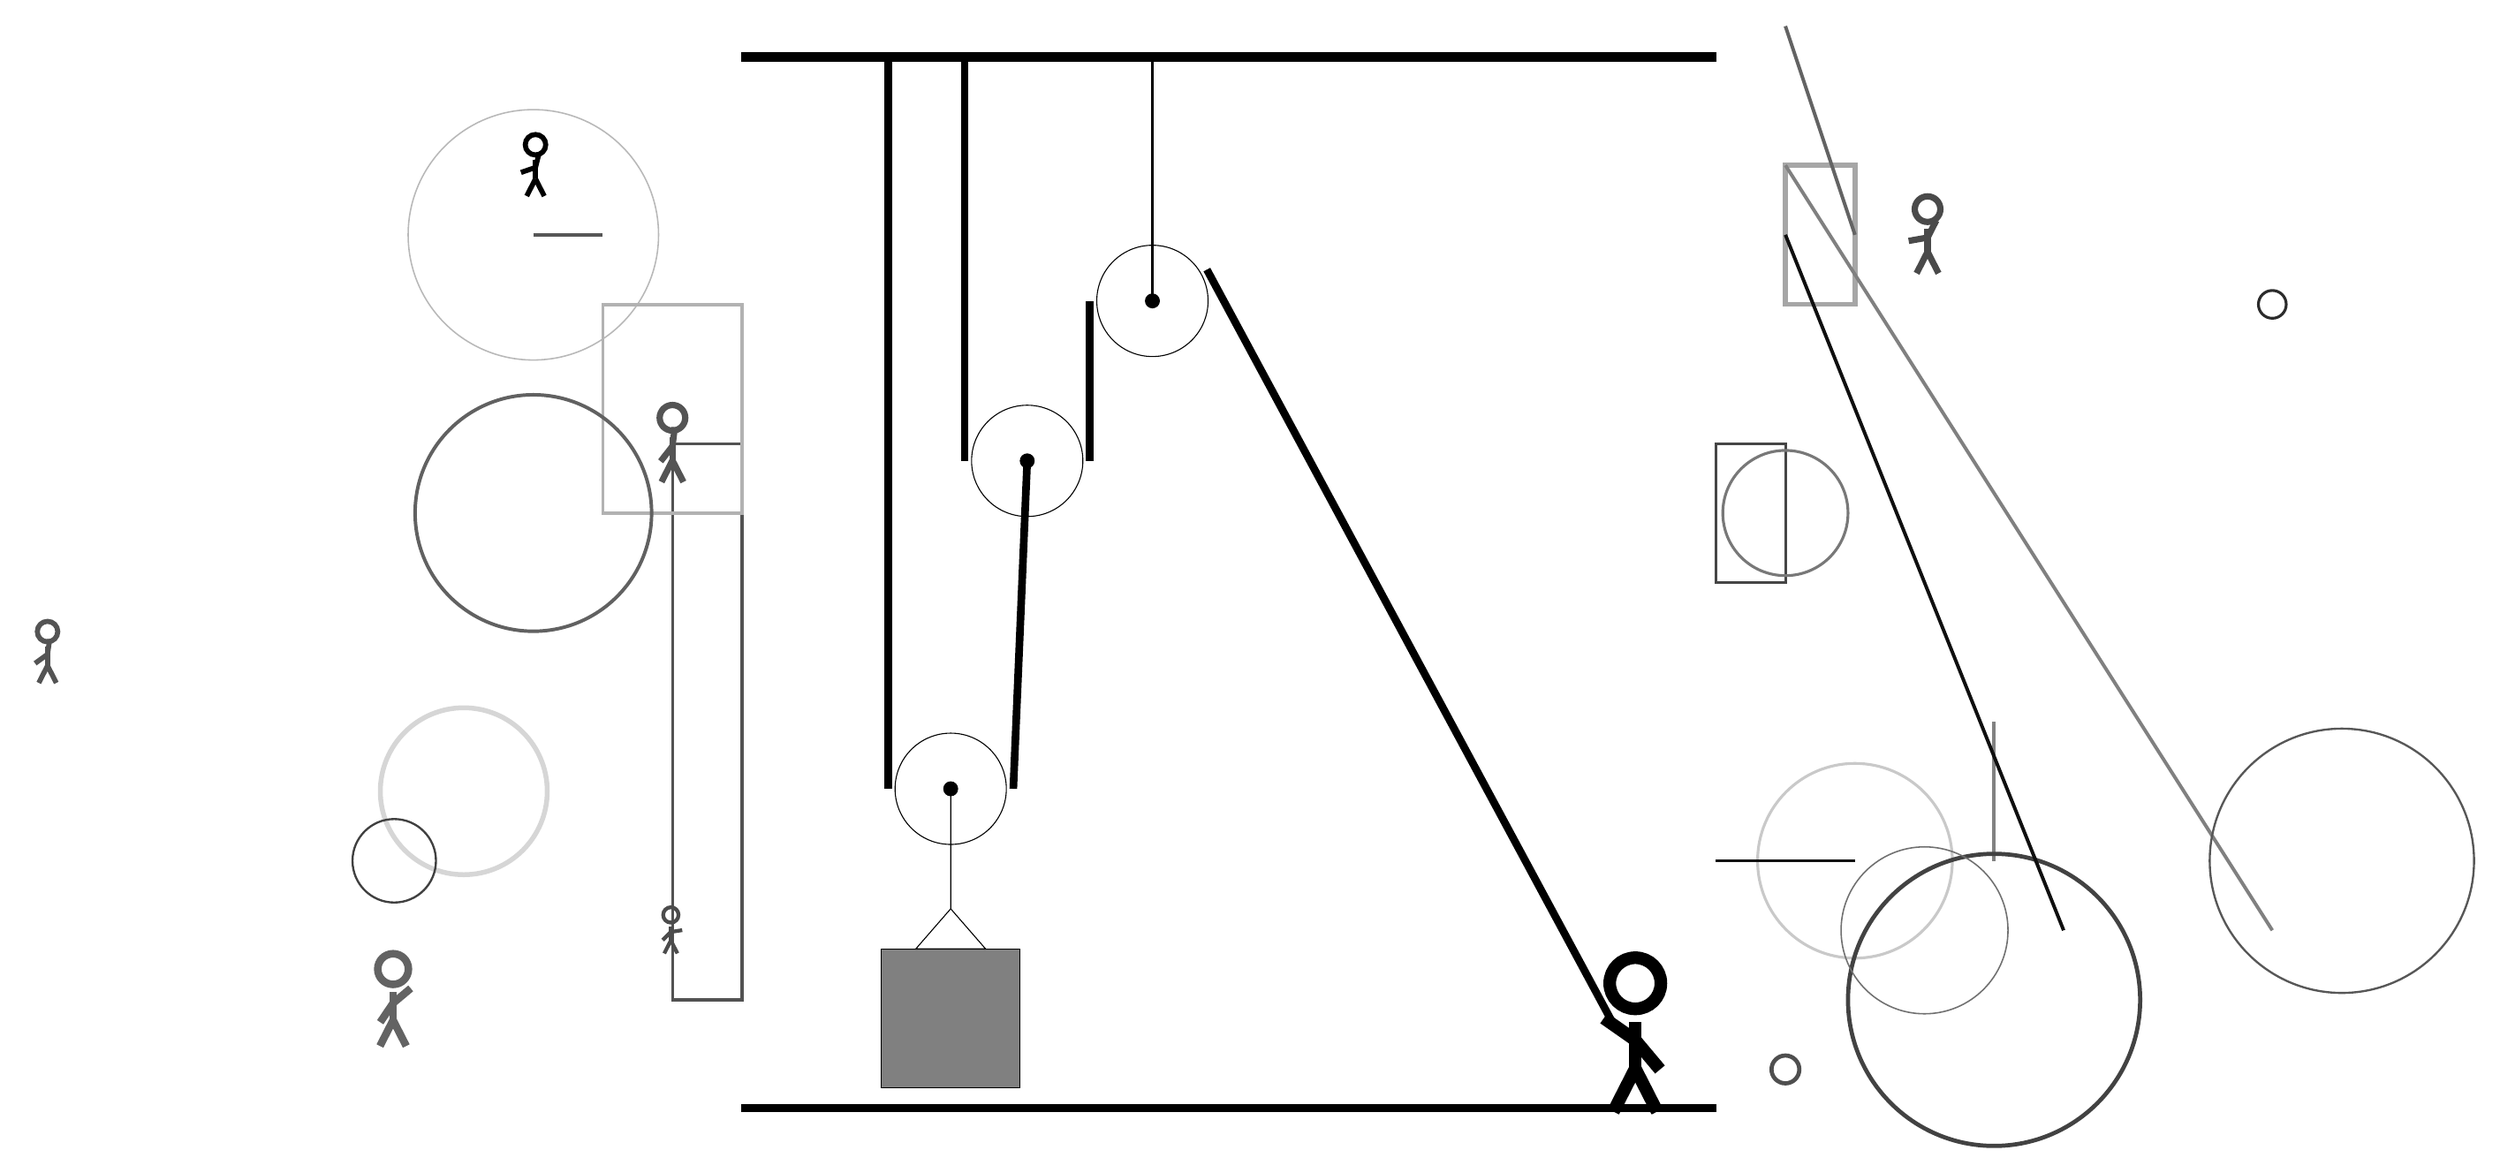
\begin{tikzpicture}
			%%%%% START %%%%%
			
			\draw[fill=black] (-2, 11.5) rectangle (12, 11.625);
			
			\draw (1, 1.035) circle (0.8);
			\draw[fill=black] (1, 1.035) circle (0.1);
			
			\draw (2.1, 5.75) circle (0.8);
			\draw[fill=black] (2.1, 5.75) circle (0.1);
			
			\draw (3.9, 8.05) circle (0.8);
			\draw[fill=black] (3.9, 8.05) circle (0.1);
			\draw[thick] (3.9, 8.05) -- (3.9, 11.5);
			
			\draw (1, 1.035) -- (1, -0.69) -- (0.5, -1.265) -- (1.5, -1.265) -- (1, -0.69);
			\draw[fill=black!50] (0, -1.265) rectangle (2, -3.265);
			
			\draw[line width=1.1mm] (0.1, 11.5) -- (0.1, 1.035);
			\centerarc[line width=1.1mm](1, 1.035)(180:360:0.9);
			\draw[line width=1.1mm](1.9, 1.035) -- (2.1, 5.75);
			\draw[line width=1.1mm] (1.2, 11.5) -- (1.2, 5.75);
			\centerarc[line width=1.1mm](2.1, 5.75)(180:360:0.9);
			\draw[line width=1.1mm](3.0, 5.75) -- (3.0, 8.05);
			\centerarc[line width=1.1mm](3.9, 8.05)(30:180:0.9);
			\draw[line width=1.1mm] (4.683, 8.5) -- (10.5, -2.3);
			
			\draw[line width=0.4mm, color=black!73] (13, 4) rectangle (12, 6);
			
			\draw[line width=0.7mm, color=black!35] (14, 10) rectangle (13, 8);
			\draw[line width=0.4mm, color=black!68] (-2, 6) rectangle (-3, -2);
			\draw[line width=0.5mm, color=black!61](13, 12) -- (14, 9);
			\draw[line width=0.5mm, color=black!49](16, 2) -- (16, 0);
			\draw [line width=0.4mm, color=black!83](20, 8) circle (0.2);
			\draw [line width=0.2mm, color=black!28](-5, 9) circle (1.8);
			\draw [line width=0.4mm, color=black!53](13, 5) circle (0.9);
			\node[line width=0.7mm, color=black!100] at (-5, 10) {\Strichmaxerl[4][19][76]};
			
			\draw[line width=0.5mm, color=black!30] (-4, 5) rectangle (-2, 8);
			\node[line width=0.3mm, color=black!67] at (-3, 6) {\Strichmaxerl[5][52][83]};
			\draw [line width=0.4mm, color=black!21](14, 0) circle (1.4);
			\draw [line width=0.6mm, color=black!74](16, -2) circle (2.1);
			\node[line width=0.4mm, color=black!70] at (-3, -1) {\Strichmaxerl[3][45][9]};
			\node[line width=0.6mm, color=black!71] at (15, 9) {\Strichmaxerl[5][10][63]};
			\draw [line width=0.7mm, color=black!16](-6, 1) circle (1.2);
			\draw [line width=0.2mm, color=black!56](15, -1) circle (1.2);
			\draw[line width=0.5mm, color=black!66](-5, 9) -- (-4, 9);
			\draw [line width=0.5mm, color=black!62](-5, 5) circle (1.7);
			\node[line width=0.4mm, color=black!67] at (-12, 3) {\Strichmaxerl[4][36][82]};
			\draw[line width=0.5mm, color=black!50](13, 10) -- (20, -1);
			
			\draw [line width=0.3mm, color=black!66](21, 0) circle (1.9);
			\draw [line width=0.3mm, color=black!75](-7, 0) circle (0.6);
			\node[line width=0.4mm, color=black!61] at (-7, -2) {\Strichmaxerl[6][56][40]};
			\draw[line width=0.5mm, color=black!94](14, 0) -- (12, 0);
			\draw [line width=0.6mm, color=black!69](13, -3) circle (0.2);
			
			\draw[line width=0.5mm, color=black!94](13, 9) -- (17, -1);
			
			\node at (10.8, -2.5) {\Strichmaxerl[10][-35][-50]};
			
			\draw[fill=black] (-2, -3.5) rectangle (12, -3.6);
			
			%%%%% END %%%%%
		\end{tikzpicture}
	\end{figure}	
\end{document}